\documentclass[11pt]{article}
\usepackage[margin=1in]{geometry}
\usepackage{graphicx} % Required for inserting images
\usepackage{amsmath,amssymb}
\usepackage{booktabs}
\usepackage{tabularx}
\usepackage{enumitem}
\usepackage{algorithm}
\usepackage{algpseudocode}
\usepackage{listings}
\usepackage{xcolor}
\usepackage[most]{tcolorbox}
\usepackage[hidelinks]{hyperref}

\lstset{
  basicstyle=\ttfamily\small,
  keywordstyle=\bfseries,
  commentstyle=\itshape\color{gray},
  columns=fullflexible,
  frame=single,
  breaklines=true,
  language=C++
}

% Marks items the authors must confirm before submission.
\newcommand{\todo}[1]{\textcolor{red}{[TODO: #1]}}

% "In plain words" boxes for readers new to the biology or quantum parts.
\newtcolorbox{plain}{colback=blue!4,colframe=green!45!black,
  fonttitle=\bfseries,title=In plain words,breakable}

\title{MSARCH -- Project Specifications\\[4pt]
\large GPU-Accelerated Network Screening for Alzheimer's Disease\\
Drug Repurposing, with an Optional Simulated-Quantum Drug-Combination Benchmark}
\date{September 2026}

\begin{document}

\maketitle

    \begin{abstract}
Developing a new Alzheimer's disease (AD) drug takes more than a decade, and almost all candidates fail. \emph{Drug repurposing}---finding already-approved drugs that might also help AD---is a faster route. A well-established way to screen for such drugs treats the cell's proteins as a graph: a drug is a promising candidate if the proteins it acts on sit unusually close, in shortest-path distance, to the proteins linked to AD. Deciding what ``unusually close'' means requires comparing each drug against thousands of random look-alikes, which makes the screen expensive. We propose a CUDA implementation of this screen. It computes all shortest-path distances on the human protein-interaction network with a bit-parallel breadth-first search, then scores every drug against thousands of random samples in parallel on the GPU. We compare its execution time against a sequential C++ version, check that both produce identical distances, and test whether the resulting ranking places drugs that have already entered AD clinical trials near the top. As an optional extension, we express the choice of a small drug combination as a Quadratic Unconstrained Binary Optimization (QUBO) problem and benchmark an exact GPU brute-force solver and classical heuristics against the Quantum Approximate Optimization Algorithm (QAOA), simulated on the GPU with NVIDIA cuQuantum (no quantum hardware is used).
\end{abstract}
    \section{Introduction}

\subsection{Why Alzheimer's disease needs faster drug discovery}

Alzheimer's disease (AD) is the most common cause of dementia. In the brain it shows two hallmarks: clumps of a protein fragment called amyloid-$\beta$ that build up between nerve cells (plaques), and twisted fibers of a protein called tau inside nerve cells (tangles). Over years, nerve cells stop working and die, and memory and thinking decline.

Developing a brand-new drug from scratch takes more than ten years, and AD has one of the highest failure rates of any disease area. \textbf{Drug repurposing} offers a shortcut: take a drug that is already approved for something else (so its safety in humans is known) and test whether it could also help AD. The hard part is choosing which of the thousands of existing drugs deserve a closer look. That choice is what computation can help with.

\subsection{Thinking of the cell as a graph}

Proteins are the molecular machines that do most of the work in a cell, and they rarely work alone: they bind to and act on each other. If we draw every human protein as a node and every known physical interaction between two proteins as an edge, we get the \textbf{human protein--protein interaction network}, or \emph{interactome}: a graph with roughly 15{,}000--18{,}000 nodes and about 150{,}000 to 700{,}000 edges, depending on the database.

Two ideas from \emph{network medicine}~\cite{barabasi2011network} make this graph useful:
\begin{enumerate}[nosep]
  \item Proteins linked to the same disease tend to cluster in the same neighborhood of the graph, forming a \emph{disease module}~\cite{menche2015uncovering}. For AD, the starting points are genes identified by large genetic studies~\cite{bellenguez2022new}.
\begin{figure}[h]
    \centering
    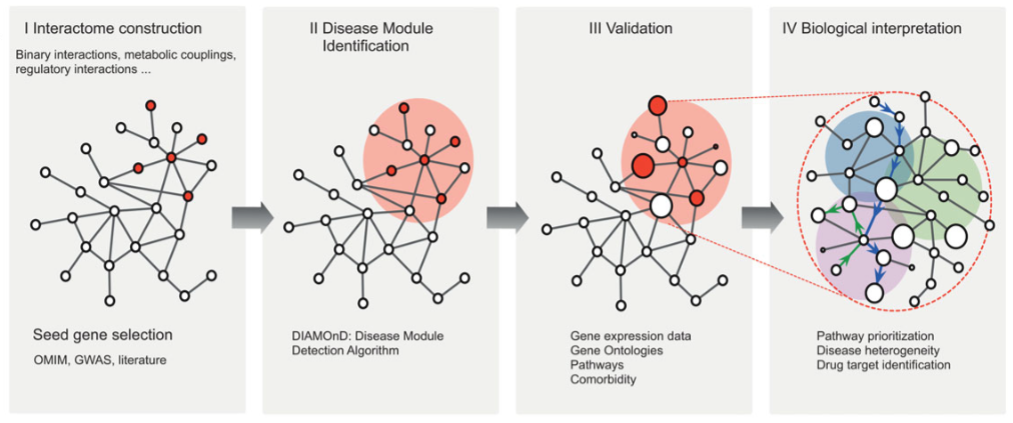
\includegraphics[width=0.5\linewidth]{images/network_module.png}
    \caption{Example of identifying a network module}
    \label{fig:example of a network module}
\end{figure}
    
  \item Most drugs work by binding to one or a few proteins, called the drug's \emph{targets}. A drug whose targets sit close to the disease module is more likely to affect the disease~\cite{guney2016network}.
\begin{figure}[h]
    \centering
    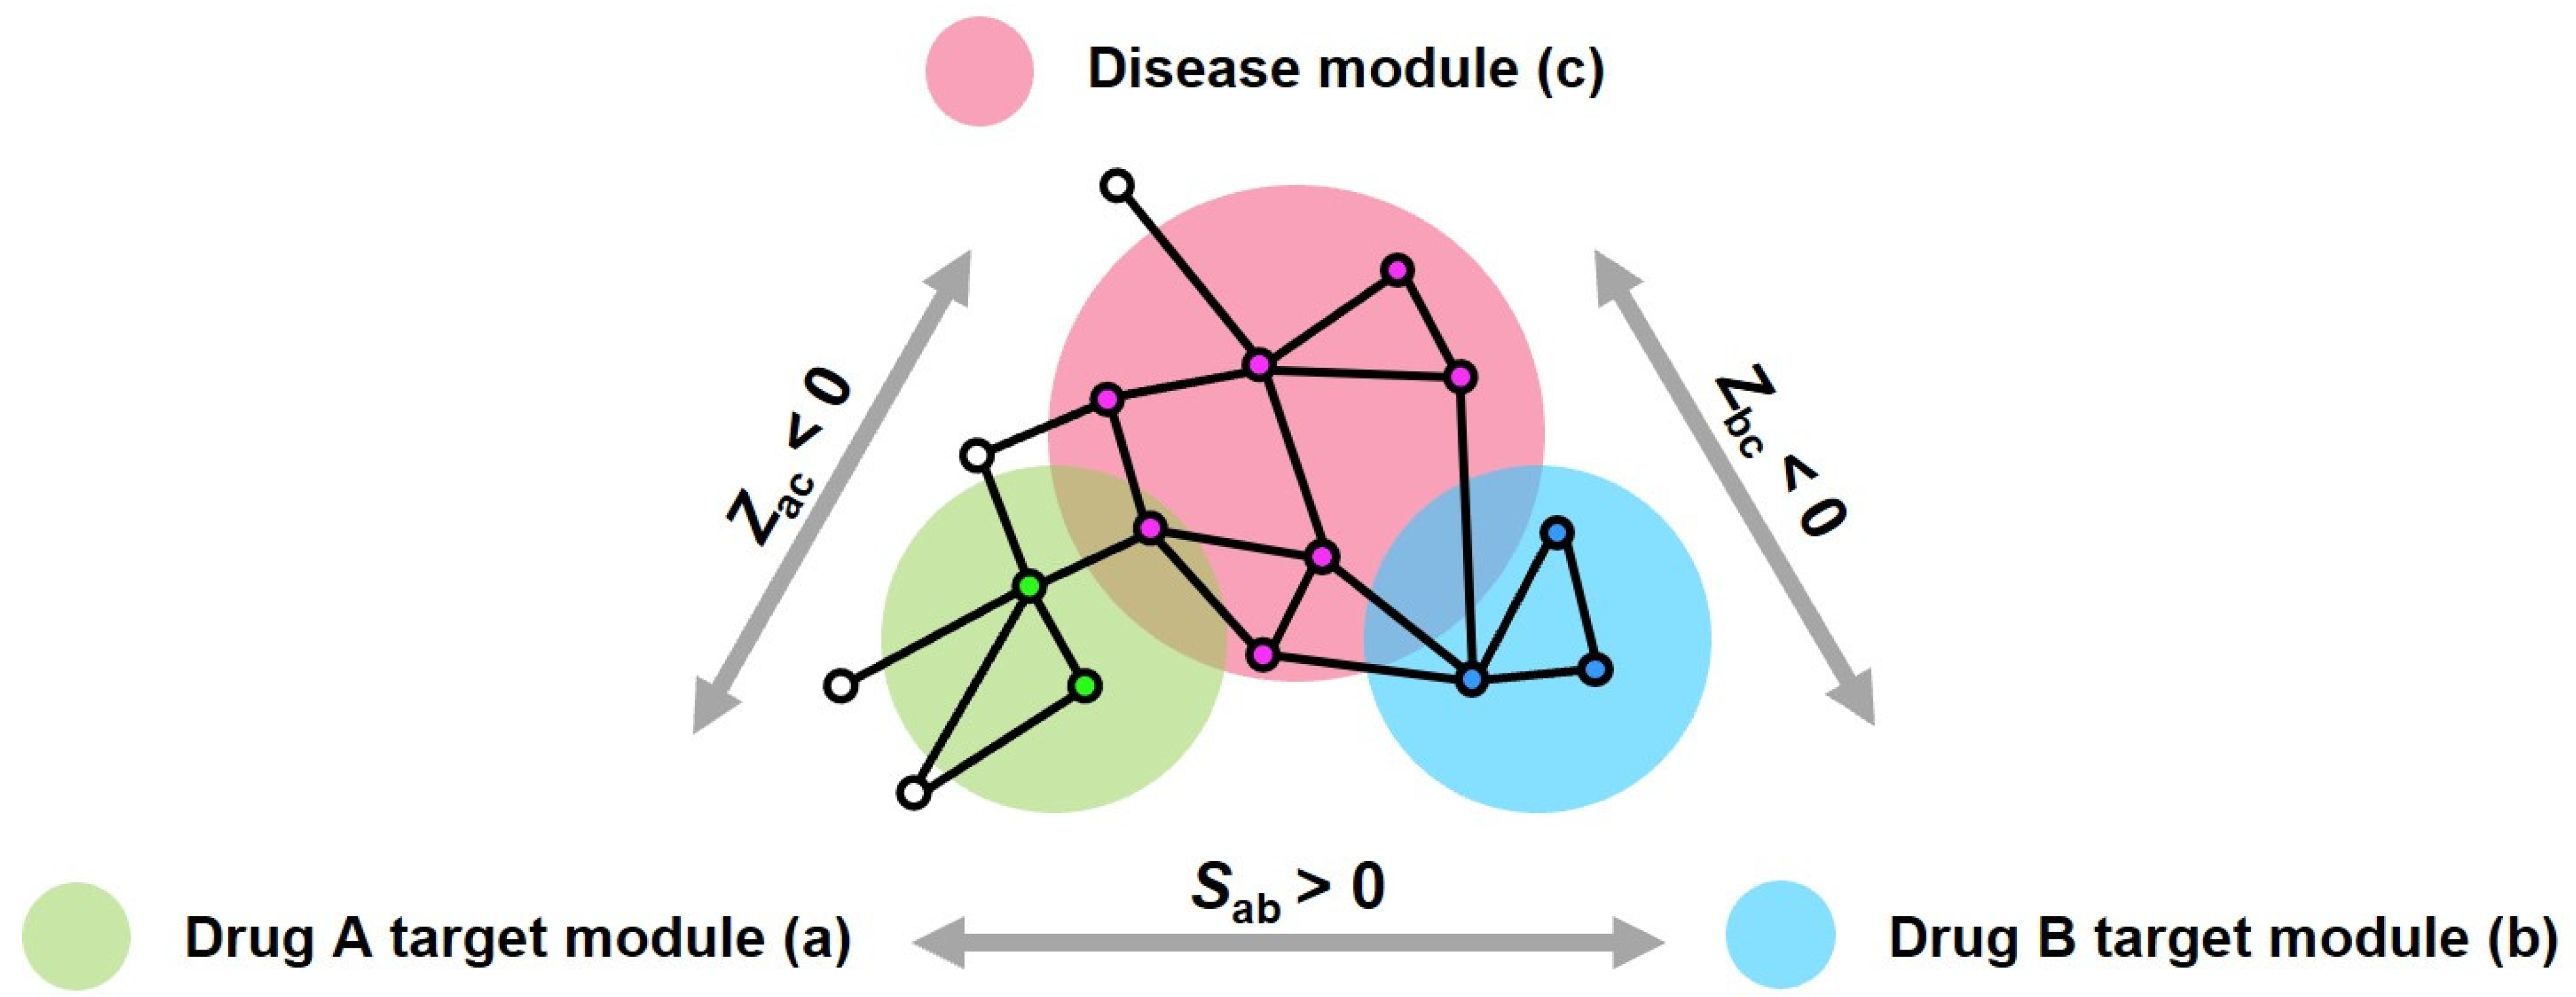
\includegraphics[width=0.5\linewidth]{images/network_drug.png}
    \caption{Example of a drug targeting a disease module}
    \label{fig:enter-label}
\end{figure}
\end{enumerate}

This approach has already produced testable AD hypotheses: network screening combined with analysis of patient insurance records pointed to sildenafil as an AD candidate~\cite{fang2021endophenotype}, and recent pipelines rank drugs for different stages of AD~\cite{csbj2023proximity} or also screen out drugs with heart-rhythm risks~\cite{lqt2025proximity}.

\subsection{Why this is a computer architecture problem}

Distance has to be judged fairly. Hub proteins with many connections are close to almost everything, so a raw distance would favor drugs that simply hit popular proteins. The standard fix~\cite{guney2016network} is to compare each drug against many random ``fake drugs'' whose targets have similar numbers of connections, and report how unusual the real distance is as a $z$-score. This creates a lot of work:
\begin{itemize}[nosep]
  \item shortest-path distances between every pair of proteins: one
        breadth-first search (BFS) from each of $\sim$15{,}000--18{,}000 nodes;
  \item for each of several thousand drugs, 1{,}000 or more random
        samples, each needing many distance look-ups;
  \item for drug combinations, the same distances between every pair of drugs.
\end{itemize}

All of these are \emph{discrete} and \emph{data-parallel}: thousands of independent BFS runs, and millions of independent random samples that each do the same look-up-and-minimum operation. That is exactly the shape of work GPUs are built for. Commonly used tools, however, are single-threaded Python scripts, which limits how many random samples, network versions, and disease modules researchers can afford to test.

\subsection{Supplementary Quantum Computation}

Once single drugs are ranked, a natural next question is which small \emph{combination} of drugs covers the disease module well without the drugs overlapping each other~\cite{cheng2019network}. Choosing the best subset from a shortlist is a yes/no decision per drug, which can be written as a Quadratic Unconstrained Binary Optimization (QUBO) problem~\cite{glover2019tutorial,lucas2014ising}. QUBOs are the standard input for quantum optimization algorithms such as QAOA~\cite{farhi2014qaoa}, which we simulate on the GPU with NVIDIA cuQuantum~\cite{bayraktar2023cuquantum}; no quantum hardware is used. Because the shortlist is small, we can also find the exact best answer by brute force on the GPU and compare QAOA with exact and classical solvers on the same biology-derived problems.

\subsection{What this project delivers}

\begin{enumerate}[nosep]
  \item A CUDA program that computes all shortest-path distances on the human
        interactome and scores every drug's closeness to the AD module.
  \item A sequential C++ version of the same steps, and an
        execution-time comparison between the two.
  \item A ranked list of repurposing candidates for AD, checked against drugs
        that have already entered AD clinical trials.
  \item (Optional) A QUBO formulation of AD drug-combination selection, and a
        benchmark of exact, classical, and GPU-simulated QAOA solvers on it.
\end{enumerate}

Section~\ref{sec:rrl} reviews related work, Section~\ref{sec:problem} states the problem and objectives, and Sections~\ref{sec:method}--\ref{sec:milestones} follow the course outline: project description, target platform, and milestones. Technical details are collected in the appendices.

    \section{Review of Related Literature}
\label{sec:rrl}

\subsection{Network medicine and the disease module}

Network medicine studies disease through the network of molecular interactions rather than one gene at a time~\cite{barabasi2011network}. Menche et al.~\cite{menche2015uncovering} showed that proteins associated with the same disease form a connected neighborhood (a \emph{disease module}) in the human interactome, even though the interactome is still incomplete. They also defined a \emph{separation} measure: two sets of proteins that overlap in the network have negative separation, and sets that are far apart have positive separation.

\subsection{Network proximity for drug repurposing}

Guney et al.~\cite{guney2016network} turned this into a drug screen. For a drug with target set $T$ and a disease module $S$, the \emph{closest distance} is the average, over the drug's targets, of the shortest-path distance to the nearest disease protein. To correct for hub proteins, they compare it with the same measure for random target and disease sets that have matching degrees, giving a $z$-score. They showed that drugs with significantly negative $z$ (closer than chance) are enriched for drugs that actually treat the disease. Cheng et al.~\cite{cheng2018network} applied the approach to cardiovascular disease and confirmed predictions with patient-record data, and later showed that good drug combinations follow a \emph{complementary exposure} pattern: both drugs are close to the disease module, but their own targets are separated from each other~\cite{cheng2019network}.

\subsection{Network proximity studies in Alzheimer's disease}

Fang et al.~\cite{fang2021endophenotype} built AD modules around amyloid and tau biology, screened drugs by proximity, and used insurance claims data to find that sildenafil users had lower AD incidence. A 2023 pipeline~\cite{csbj2023proximity} built separate modules for different pathological stages of AD and ranked candidate drugs for each, and a 2025 study~\cite{lqt2025proximity} combined proximity ranking with screening for drugs that raise the risk of a dangerous heart rhythm (Long QT syndrome). These studies establish both the method and its relevance to AD. The inputs they rely on are public: integrated knowledge graphs such as Hetionet~\cite{himmelstein2017hetionet}, interaction databases such as BioGRID~\cite{oughtred2021biogrid} and STRING~\cite{szklarczyk2023string}, drug--target databases such as ChEMBL~\cite{zdrazil2024chembl}, DGIdb~\cite{freshour2021dgidb}, and DrugBank~\cite{knox2024drugbank}, AD genes from genome-wide association studies~\cite{bellenguez2022new}, and the annual AD drug-development pipeline review~\cite{cummings2024pipeline}, which lists drugs currently in AD clinical trials.

\subsection{Graph traversal on GPUs}

Breadth-first search is the building block for shortest paths on unweighted graphs. Harish and Narayanan~\cite{harish2007accelerating} gave one of the first CUDA BFS implementations, Merrill et al.~\cite{merrill2012scalable} showed how to make GPU BFS efficient with prefix-sum-based frontier expansion, and Gunrock~\cite{wang2016gunrock} provides a general GPU graph library. When many BFS runs share one graph, \emph{multi-source BFS} (MS-BFS)~\cite{then2014more} runs up to 64 or more searches at once by storing, for each node, a bit per search; expanding the frontier then becomes bitwise OR and AND on machine words. This fits data-level parallelism well: each
thread handles one node and one word of bits, with no branching per search.

\subsection{QUBO, quantum optimization, and drug combinations}

A QUBO asks for the binary vector $x$ that minimizes a quadratic function $x^{\top}Qx$. Many selection problems can be written this way~\cite{glover2019tutorial,lucas2014ising}. QUBOs can be attacked with classical heuristics such as simulated annealing~\cite{kirkpatrick1983optimization}, with quantum annealers, or with the gate-based QAOA~\cite{farhi2014qaoa}. NVIDIA cuQuantum~\cite{bayraktar2023cuquantum} simulates quantum circuits on GPUs, which lets QAOA be tested on small problems without quantum hardware. Most relevant here, a 2026 study~\cite{qmi2026combinations} formulated network-based drug-combination prediction as a QUBO and solved it with quantum annealing.

\subsection{Synthesis and gap}

\begin{table}[h]
\centering
\small
\begin{tabularx}{\linewidth}{@{}lXccc@{}}
\toprule
Work & What it does & AD & GPU & Quantum \\
\midrule
Guney et al.~\cite{guney2016network} & Proximity $z$-score drug screen & -- & -- & -- \\
Cheng et al.~\cite{cheng2019network} & Complementary-exposure drug combinations & -- & -- & -- \\
AD proximity studies~\cite{fang2021endophenotype,csbj2023proximity,lqt2025proximity} & AD drug repurposing & \checkmark & -- & -- \\
GPU BFS / MS-BFS~\cite{merrill2012scalable,then2014more,wang2016gunrock} & Fast graph traversal & -- & \checkmark & -- \\
Quantum drug combinations~\cite{qmi2026combinations} & QUBO + quantum annealing & -- & -- & \checkmark \\
\textbf{This work} & GPU proximity screen + optional simulated-QAOA benchmark & \checkmark & \checkmark & \checkmark \\
\bottomrule
\end{tabularx}
\caption{How this project relates to prior work. \todo{Confirm from the
papers whether any of the AD studies or \cite{qmi2026combinations} used GPUs
or targeted AD.}}
\end{table}

The method (network proximity), its relevance to AD, fast GPU graph traversal, and quantum formulations of drug combinations all exist, but separately. Proximity screens are typically run as sequential scripts, which caps the number of random samples and the number of network and disease-module variants that can be compared. We found no GPU implementation of the full proximity screen, and no study benchmarking exact, classical, and simulated gate-model QAOA solvers on AD drug-combination QUBOs.

    \section{Problem Statement}
\label{sec:problem}

\subsection{Problem}

Network proximity is a proven way to shortlist drugs for repurposing, and it has been applied to Alzheimer's disease. But the screen is expensive to run properly. It needs shortest-path distances between all pairs of $\sim$15{,}000--18{,}000 proteins, and each of the $\sim$1{,}400 or more drugs must be compared against 1{,}000 or more random samples to get a fair $z$-score. Typical implementations are sequential scripts, so researchers settle for few random samples, one version of the interaction network, and one definition of the AD module---even though results can change with each of these choices.

A second, smaller problem sits on top: choosing a good \emph{combination} of drugs from the shortlist is a combinatorial selection problem. It can be written as a QUBO, the input format for quantum optimization, but it is not yet known how well a gate-based quantum algorithm (QAOA, simulated on a GPU) handles this specific AD problem compared with the exact answer and with classical solvers.

\subsection{Proposed solution}

We propose a CUDA program that runs the full proximity screen on the GPU, built as five modules with clear inputs and outputs so each can be developed and tested separately (Table~\ref{tab:modules}).

\begin{table}[h]
\centering
\small
\begin{tabularx}{\linewidth}{@{}lXXl@{}}
\toprule
Module & Input & Output & Runs on \\
\midrule
1. Data preparation & Interaction list, drug--target list, AD gene list & Graph in compressed form (CSR), target and disease sets as node IDs & CPU \\
2. All-pairs distances & Graph (CSR) & Distance matrix $D$ ($N\times N$, 1 byte per entry) & GPU \\
3. Proximity scoring & $D$, drug target sets, AD module & Proximity and $z$-score per drug & GPU \\
4. Ranking and validation & $z$-scores, list of AD trial drugs & Ranked candidates, validation metrics & CPU \\
5. Combinations (optional) & Top-$n$ drugs, $D$ & Drug--drug separation matrix, QUBO, best combination & GPU (+ cuQuantum) \\
\bottomrule
\end{tabularx}
\caption{Pipeline modules. Module 5 is optional and independent of the graded
core (Modules 1--4).}
\label{tab:modules}
\end{table}

\subsection{Research questions}

\begin{enumerate}[label=\textbf{RQ\arabic*.},leftmargin=*]
  \item How much faster is the GPU implementation than a sequential C++ implementation for the all-pairs distance step and the proximity scoring step, and how does the speedup change with network size and number of random samples?
  \item Does the GPU implementation give exactly the same distances, and the same $z$-scores when given the same random samples, as the sequential version?
  \item Does the proximity ranking place drugs that have entered AD clinical trials higher than simple baselines (random ranking, or ranking by number of targets)?
  \item (Optional) On AD drug-combination QUBOs small enough to solve exactly, how close do classical heuristics and simulated QAOA get to the true best answer under the same budget, and how do biology-derived instances compare with random ones? (Appendix~\ref{app:extension})
\end{enumerate}

\subsection{Objectives}

\paragraph{General objective.} To build and evaluate a GPU-accelerated
network proximity screen for Alzheimer's disease drug repurposing.

\paragraph{Specific objectives.}
\begin{enumerate}[nosep]
  \item Implement all-pairs shortest-path distances on the GPU using bit-parallel multi-source BFS.
  \item Implement proximity and $z$-score computation for all drugs on the GPU, with random sampling done in parallel.
  \item Implement the same steps sequentially in C++ and compare execution times.
  \item Verify that GPU and CPU results match.
  \item Rank AD repurposing candidates and measure how well the ranking recovers drugs already in AD trials.
  \item (Optional) Formulate AD drug-combination selection as a QUBO and compare GPU brute force, simulated annealing, and QAOA.
\end{enumerate}

\subsection{Scope and limitations}

\begin{itemize}[nosep]
  \item Public data only: interaction, drug--target, and AD gene databases. No patient data are used.
  \item Single GPU. The network has up to about 20{,}000 nodes, so the full distance matrix (at most 400~MB at one byte per entry) fits in GPU memory.
  \item Results are \emph{hypotheses}, not treatment recommendations. Closeness in a network does not prove a drug works; clinical evidence is outside the project's scope.
  \item The interactome is incomplete and biased toward well-studied proteins; we reduce this by comparing more than one database.
  \item The quantum part is simulation only, limited to about 20--30 drugs (one qubit each). It does not claim to be faster than classical methods; its purpose is to measure solution quality.
\end{itemize}

\subsection{Significance}

A fast screen lets researchers run the checks that are currently skipped: more random samples for stable $z$-scores, several networks, and several definitions of the AD module (for example, early-stage vs.\ late-stage genes). For the course, it is a clear case study of turning a graph problem into bitwise, data-parallel GPU work. For the optional part, it provides a realistic, biology-derived benchmark for quantum optimization.

    \section{Methodology}
\label{sec:method}
\subsection{Description of the Proposed Project}

\subsubsection{Inputs}

All inputs are public and can be downloaded at the start of the project.
\begin{itemize}
  
  \item \textbf{Primary network and drug data: Hetionet~\cite{himmelstein2017hetionet}.}
  An integrated knowledge graph from which we use three edge types: protein--protein interactions (these include the interactome of Menche et al.~\cite{menche2015uncovering}), DrugBank-derived drug--target links, and disease--gene links for Alzheimer's disease. The processed network has $N=15{,}139$ proteins and $E=147{,}149$ edges, with 1{,}383 drugs that have at least one target in the network and 185 AD genes. Edges are unweighted and undirected. Hetionet combines sources with mixed licenses, some non-commercial, so we do not redistribute raw data  as illustrated in \ref{fig:example of a network module}).
\begin{figure}[h]
    \centering
    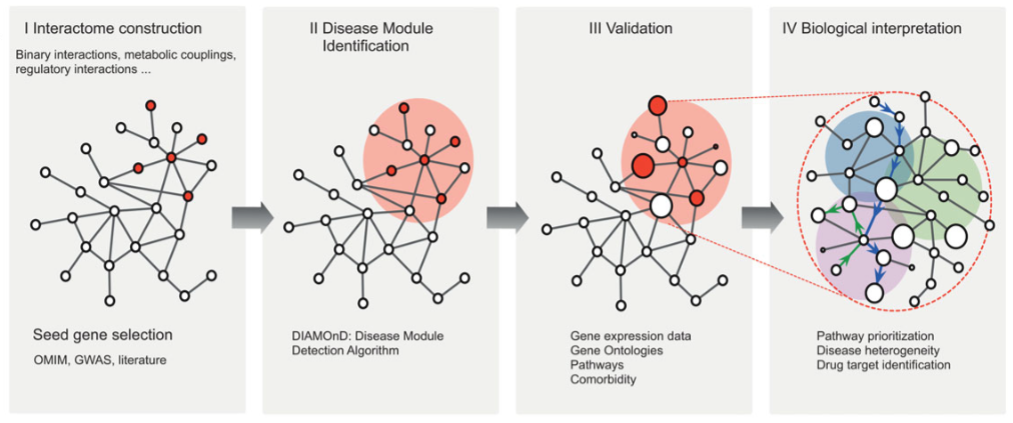
\includegraphics[width=0.5\linewidth]{images/network_module.png}
    \caption{Example of identifying a network module}
    \label{fig:example of a network module}
\end{figure}
  
  \item \textbf{Comparison network: BioGRID~\cite{oughtred2021biogrid}.} Human physical interactions: $N=17{,}602$ and $E=679{,}846$ (about 4.6 times as many edges), with 1{,}382 drugs and 191 AD genes mapped. It is the heavier workload for the timing experiments. STRING~\cite{szklarczyk2023string} at several confidence cut-offs is an optional further comparison, and  ChEMBL~\cite{zdrazil2024chembl} or DGIdb~\cite{freshour2021dgidb} drug--target data can replace the DrugBank-derived links as a robustness check as illustrated in  \ref{fig:disease-module}).
\begin{figure}[h]
    \centering
    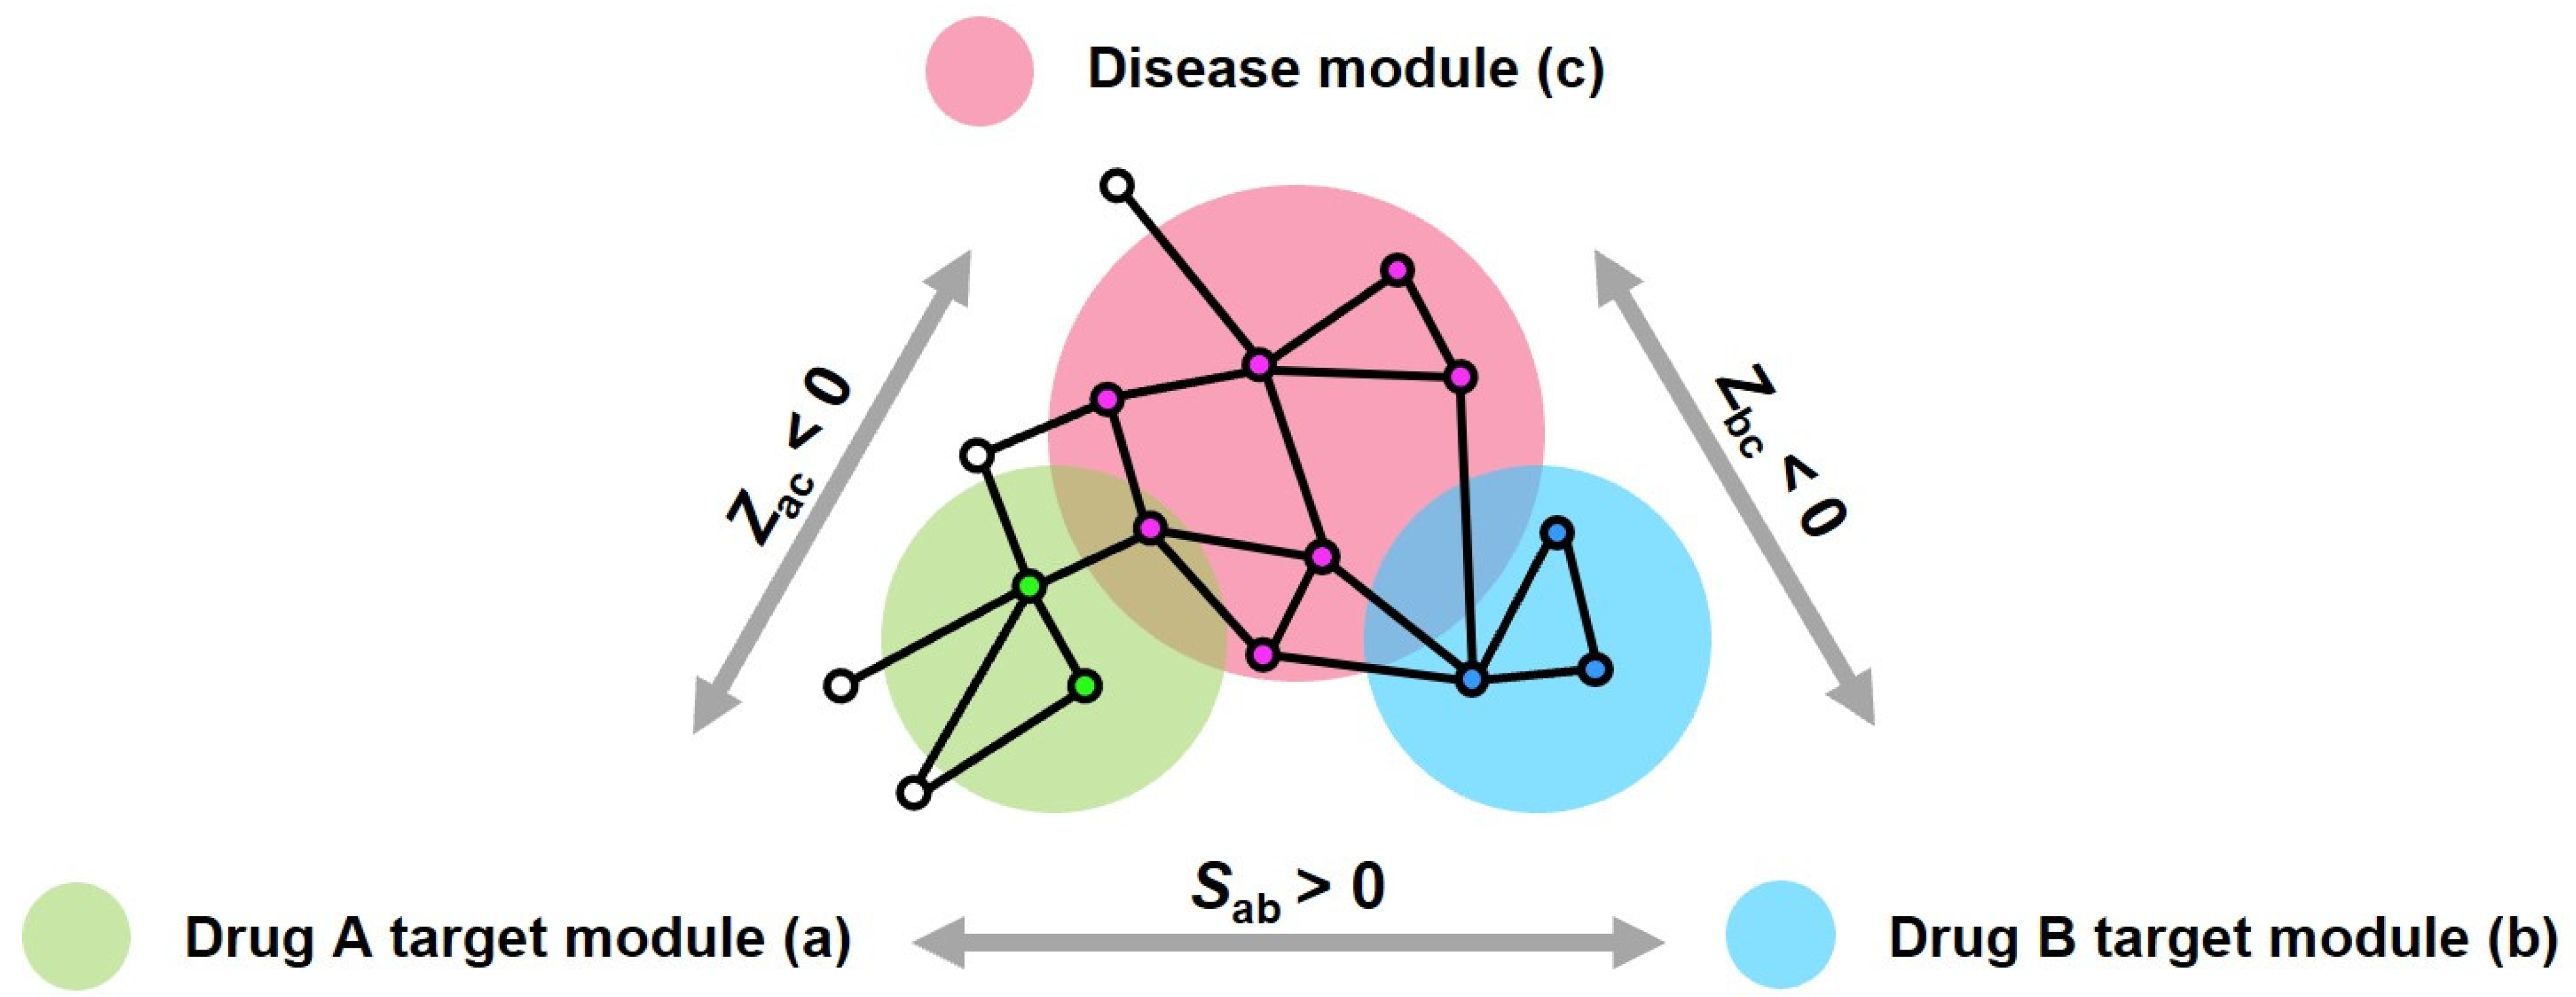
\includegraphics[width=0.5\linewidth]{images/network_drug.png}
    \caption{Example of a drug targeting a disease module}
    \label{fig:disease-module}
\end{figure}
  
  \item \textbf{AD disease module.} Hetionet's disease--gene links for Alzheimer's disease (185 proteins). An alternative module built from the largest recent genetic study~\cite{bellenguez2022new} plus well-known AD genes (e.g., \textit{APP}, \textit{PSEN1}, \textit{PSEN2}, \textit{APOE}, \textit{MAPT}) is a robustness variant.
  
  \item \textbf{Validation list.} About 30 drugs that have entered AD clinical trials. The list was compiled from general knowledge and \textbf{must be verified} against ClinicalTrials.gov and the annual AD drug-development pipeline review~\cite{cummings2024pipeline} before any result is reported. 
  
  \item \textbf{Parameters.} Number of random samples per drug $R\in\{100, 1{,}000, 10{,}000\}$, and, for the optional part, shortlist size $n\le 28$ and combination size $k$.
\end{itemize}

The GPU only ever sees three things: a graph (who connects to whom), a few
thousand small lists of node IDs (each drug's targets), and one more list of
node IDs (the AD module). Everything biological is just labels on those
node IDs.

\subsubsection{Proposed Process}

The screen answers one question for every drug: \emph{are this drug's targets
closer to the AD module than we would expect by chance?}

\begin{enumerate}
  \item \textbf{Distance.} For each target of the drug, find the shortest
        path (fewest edges) to the nearest AD protein, and average these over
        the drug's targets. This is the drug's \emph{proximity} $d$; smaller
        means closer.
  \item \textbf{Chance level.} Repeat the same calculation $R$ times using
        random ``fake'' target sets and random ``fake'' AD modules of the same
        sizes, where each random protein is picked to have a similar number
        of connections as the real one it replaces. This gives the average
        $\mu$ and spread $\sigma$ of proximity by chance.
  \item \textbf{Score.} $z = (d-\mu)/\sigma$. A strongly negative $z$ (for
        example $z < -2$) means the drug is unusually close to AD.
\end{enumerate}

\paragraph{(i) Processes parallelized with SIMT (GPU/CUDA).}
\begin{enumerate}
  \item \textbf{All-pairs shortest-path distances.} One BFS from every node gives the full distance matrix $D$, where $D[a][b]$ is the number of steps from protein $a$ to protein $b$. Since distances in this network are small (rarely above 15), each entry fits in one byte. We run many BFS searches at once using \emph{bit-parallel multi-source BFS}~\cite{then2014more}: each node keeps one bit per search, so a 64-bit word tracks 64 searches, and one step of all 64 searches becomes a bitwise OR over the node's neighbors.
  \item \textbf{Proximity and random sampling .} Every (drug, random sample) pair is independent. Each GPU thread generates one random sample, looks up the needed distances in $D$, takes minimums and an average, and a block-level reduction combines the samples into $\mu$ and $\sigma$ for that drug.
  % \item \textbf{Drug--drug separation } For the shortlist, the distance-based separation between every pair of drugs, computed with the same look-up-and-minimum pattern.
  % \item \textbf{Exact QUBO solver (Module 5, optional).} Tries all $2^n$ yes/no choices for $n$ shortlisted drugs, one GPU thread per group of choices; practical up to $n\approx 30$.
  % \item \textbf{QAOA simulation (Module 5, optional).} Simulated with cuQuantum's cuStateVec, which itself runs data-parallel over the $2^n$ numbers that describe the quantum state.
\end{enumerate}

\paragraph{(ii) Related works and how this implementation differs.}
Network proximity for drug repurposing was introduced by Guney et al.~\cite{guney2016network} and has been applied to AD several times~\cite{fang2021endophenotype,csbj2023proximity,lqt2025proximity}. These studies focus on the biology and generally run the screen as sequential scripts. GPU BFS is well studied~\cite{harish2007accelerating,merrill2012scalable,wang2016gunrock}, and bit-parallel MS-BFS was designed for running many searches over one graph~\cite{then2014more}, but these are general-purpose graph tools, not proximity screens. 
% Quantum drug-combination selection was recently formulated as a QUBO and solved with quantum annealing~\cite{qmi2026combinations}.

Our implementation differs in that it:
\begin{itemize}[nosep]
  \item runs the \emph{whole} screen on the GPU, including the random sampling, which is usually the slowest part;
  \item stores distances as one byte each and produces them with bitwise MS-BFS, so the full matrix for 20{,}000 proteins (400~MB) stays on the GPU and every later step is a fast memory look-up;
  \item uses the same counter-based random number generator on CPU and GPU, so both versions draw identical random samples and their results can be compared exactly;
  \item targets AD specifically and checks results against AD trial drugs;
  % \item (Optional) benchmarks simulated gate-based QAOA against the exact optimum and classical solvers on the same biology-derived instances, instead of reporting a quantum solution alone.
\end{itemize}

\paragraph{(iii) Parallelization plan.}
\begin{center}
\small
\begin{tabularx}{\linewidth}{@{}lXl@{}}
\toprule
Step & How work is split across GPU threads & Limited by \\
\midrule
Multi-source BFS & Sources processed in batches of $64\times W$ (e.g., 1{,}024). One thread per (node, 64-bit word). Each level: OR the neighbors' frontier words, AND with NOT-visited, write the level number into $D$ for newly reached sources. Graph stored in CSR form. Repeat until no bits change. & Memory \\
Writing $D$ & Threads for neighboring nodes write neighboring bytes of the same row of $D$, so writes are coalesced. & Memory \\
Proximity + $z$-score & One thread block per drug; each thread handles several random samples; degree-matched sampling from per-degree-bin node lists; distances read from $D$ (reads are scattered, so L2 cache matters); block reduction for $\mu$, $\sigma$. & Memory \\
Drug--drug separation & One thread per drug pair on the shortlist; same look-up pattern. & Memory \\
% QUBO brute force & One thread per block of $2^{m}$ bit patterns; patterns visited in Gray-code order so each step flips one bit and updates the cost in $O(n)$; warp and block minimum reduction. & Compute \\
\bottomrule
\end{tabularx}
\end{center}
Data moves to the GPU once (the graph and ID lists, a few MB) and results come back once ($z$-scores; $D$ only if needed).

\paragraph{(iv) Processes not parallelized.}
\begin{itemize}[nosep]
  \item Downloading and reading the databases; converting between gene and protein identifiers; removing duplicates and self-loops.
  \item Building the CSR graph and keeping its largest connected component.
  \item Grouping proteins into degree bins for the random sampling.
  \item Ranking drugs, computing validation metrics, and plotting.
  % \item Building the QUBO matrix from the separation results, and the classical optimizer loop that tunes QAOA's parameters.
\end{itemize}

\subsubsection{Outputs}

\begin{enumerate}
  \item \textbf{Distance matrix} $D$ for the interactome (binary file, one byte per entry), plus summary statistics (e.g., distance histogram).
  \item \textbf{Ranked drug list} with proximity $d$, $z$-score, and $p$-value for every drug, and the top AD repurposing candidates.
  \item \textbf{Execution-time comparison}: sequential C++ vs.\ CUDA time for (a) all-pairs distances and (b) proximity scoring, across network sizes $N$ and random-sample counts $R$, with speedup charts.
  \item \textbf{Correctness report}: GPU and CPU distance matrices are identical, and $z$-scores match when using the same random samples.
  \item \textbf{Validation}: how highly AD trial drugs are ranked, compared with simple baselines.
  % \item \textbf{(Optional) Combination results}: best $k$-drug combinations from the shortlist, and each solver's solution quality (including simulated QAOA) compared with the exact answer.
\end{enumerate}

%======================================================================
\section{Proposed Target Implementation Platform}
\label{sec:platform}

\begin{center}
\small
\begin{tabularx}{\linewidth}{@{}lX@{}}
\toprule
Component & Specification \\
\midrule
Parallel paradigm & SIMT on NVIDIA GPUs via CUDA C++ (primary); AVX2 SIMD on the CPU as a baseline; hand-written AVX-512/assembly only as an optional extra \\
GPU & NVIDIA GeForce GTX 1660: Turing (TU116), compute capability 7.5, 1{,}408 CUDA cores, 6 GB GDDR5 on a 192-bit bus, 192 GB/s \cite{gtx1660_specs}. GeForce cards are slow at 64-bit floating point, so all GPU code uses 32-bit integers (deterministic mode) or 32-bit floats. \\
CPU (baselines) & Processor	AMD Ryzen 5 3500 6-Core Processor, 3600 Mhz, 6 Core(s), 6 Logical Processor(s); Cache: L1 cache: 384KB, L2 cache: 3.0 MB, L3: 16.0 MB; RAM: 16GB. Must support AVX2 and FMA; AVX-512 is not assumed. Same machine as the GPU. \\
OS & Linux (Ubuntu 22.04/24.04), or Windows with WSL2 \\
GPU libraries & CUDA Toolkit 12.x, CUB (block reductions), a counter-based RNG (Philox, as in cuRAND/Random123) shared with the CPU code\\ % cuQuantum (cuStateVec) through CUDA-Q for the optional part \\
Languages and build & C++17 and CMake for the core; Python 3.11+ (pandas, NumPy, SciPy, matplotlib) for data preparation, validation, and plots; NetworkX as an independent reference on small graphs \\
Profiling & Nsight Systems and Nsight Compute \\
Repository & GitHub: source, build and benchmark scripts, the discussion of the parallel algorithms, and the sequential-vs-parallel timing results required for Milestone~3 \\
\bottomrule
\end{tabularx}
\end{center}

%======================================================================
\section{Mid-Project Milestones}
\label{sec:milestones}

\paragraph{Milestone 2 (Week 10) deliverable.} A live demo on the Hetionet
interactome that shows:
\begin{enumerate}[nosep]
  \item the GPU multi-source BFS producing the full distance matrix, and a check that it is identical to the sequential C++ result;
  \item the GPU proximity and $z$-score step for all drugs with $R=1{,}000$ random samples;
  \item a first sequential-vs-parallel timing table for both steps;
  \item a first ranked list of AD candidates.
\end{enumerate}

The full schedule is in Table~\ref{tab:schedule}.

\begin{table}[h]
\centering
\small
\begin{tabularx}{\linewidth}{@{}lX@{}}
\toprule
Week & Work \\
\midrule
6 & Proposal submission (Milestone 1). Download and freeze data versions. Set up repository and CMake build. \\
7 & Data preparation (identifier mapping, CSR graph, degree bins). Sequential C++ BFS and proximity; check against NetworkX on a small graph. \\
8 & GPU multi-source BFS; exact comparison with the CPU distance matrix. \\
9 & GPU proximity and $z$-score kernel with shared RNG; timing harness (CUDA events, median of 10 runs). \\
10 & \textbf{Milestone 2: mid-project demo} (above). \\
11 & Scaling experiments (Hetionet vs.\ BioGRID, optionally STRING cut-offs; $R$ up to 10{,}000); profiling; validation against AD trial drugs and baselines. \\
% 12 & (Optional) Drug--drug separation, QUBO, GPU brute force, classical heuristics, and simulated QAOA via CUDA-Q (benchmark, Appendix). \\
13 & \textbf{Milestone 3}: final GitHub submission with source, parallel-algorithm discussion, and sequential-vs-parallel timing; demo; optional conference paper. \\
\bottomrule
\end{tabularx}
\caption{Project schedule by academic week.}
\label{tab:schedule}
\end{table}
   % Sections 4-6: Methodology, Platform, Milestones
    % References (course outline item 4). Swap to IEEEtran if your TeX install has it.
    \bibliographystyle{ieeetr}
    \bibliography{refs}

    \appendix
    \section{Formal Definitions}
\label{app:math}

Let $G=(V,E)$ be the interactome with $N=|V|$ nodes, and $d(u,v)$ the shortest-path length (number of edges) between $u$ and $v$.

\paragraph{Closest distance.} For a drug with target set $T$ and disease module
$S$~\cite{guney2016network}:
\begin{equation}
  d_c(S,T) = \frac{1}{|T|}\sum_{t\in T}\min_{s\in S} d(s,t).
\end{equation}

\paragraph{Degree-matched randomization.} Nodes are grouped into bins of similar degree, each bin holding at least $b_{\min}$ nodes (e.g., 100). A random sample replaces every node of $T$ and of $S$ by a uniformly drawn node from the same bin. Over $R$ samples, with mean $\mu$ and standard deviation
$\sigma$ of $d_c$,
\begin{equation}
  z = \frac{d_c(S,T)-\mu}{\sigma},
\end{equation}
with an empirical one-sided $p$-value $p = (1+\#\{r: d_c^{(r)}\le d_c\})/(1+R)$.

\paragraph{Separation.} For two node sets $A$ and
$B$~\cite{menche2015uncovering},
\begin{equation}
  s_{AB} = \langle d_{AB}\rangle - \frac{\langle d_{AA}\rangle + \langle d_{BB}\rangle}{2},
\end{equation}
where $\langle d_{AA}\rangle$ is the mean over $a\in A$ of the distance to the nearest \emph{other} member of $A$, and $\langle d_{AB}\rangle$ is the mean, over all nodes of $A$ and $B$, of the distance to the nearest node of the other set. $s_{AB}<0$ means the two target sets overlap in the network.

\paragraph{Complementary exposure.} A drug pair is favored when both drugs are close to the disease ($z<0$) and their target sets are separated ($s_{AB}\ge0$)~\cite{cheng2019network}.

\paragraph{Combination QUBO (optional).} For a shortlist of $n$ drugs with $x_i=1$ if drug $i$ is chosen, let $w_i=-z_i>0$ reward disease proximity and $P_{ij}=\max(0,-s_{ij})$ penalize overlapping target sets. Choosing $k$ drugs:
\begin{equation}
  \min_{x\in\{0,1\}^n}\; -\sum_i w_i x_i + \lambda\sum_{i<j}P_{ij}x_ix_j
  + A\Big(\sum_i x_i - k\Big)^2 .
\end{equation}
Expanding with $x_i^2=x_i$ gives $x^{\top}Qx$ (upper-triangular form) plus the constant $Ak^2$, with
\begin{equation}
  Q_{ii} = -w_i + A(1-2k), \qquad Q_{ij} = \lambda P_{ij} + 2A \quad (i<j).
\end{equation}
$A$ must be large enough that violating the cardinality constraint never pays off (e.g., $A > \max_i w_i + \lambda\sum_j P_{ij}$); $\lambda$ is swept to show the trade-off between proximity and overlap.

%======================================================================
\section{Kernel Design Details}
\label{app:kernels}

\subsection{Data layout}

\begin{itemize}[nosep]
  \item Graph: CSR arrays \texttt{rowptr} ($N+1$ ints) and \texttt{col} ($2E$ ints).
  \item Distance matrix: $D$ as \texttt{uint8\_t}, row-major, $N^2$ bytes (324~MB at $N=18{,}000$); 255 marks ``unreachable''.
  \item MS-BFS state per batch: \texttt{seen}, \texttt{frontier}, \texttt{next}, each $N\times W$ 64-bit words ($W=16$ gives 1{,}024 sources per batch; 3 arrays $\times$ 18{,}000 $\times$ 16 $\times$ 8~B $\approx$ 7~MB).
  \item Target sets and the disease module: flattened index arrays with offsets; degree bins: node lists per bin, plus a node-to-bin map.
\end{itemize}

\subsection{Bit-parallel multi-source BFS}

\begin{algorithm}[h]
\caption{One batch of MS-BFS (sources $s_0,\dots,s_{64W-1}$)}
\begin{algorithmic}[1]
\State $\text{seen}[s_j] \gets \text{frontier}[s_j] \gets$ bit $j$ set; $D[s_j][s_j]\gets 0$
\For{$\ell = 1, 2, \dots$}
  \ForAll{nodes $v$ and words $w$ \textbf{in parallel}} \Comment{one thread per $(v,w)$}
    \State $m \gets 0$
    \ForAll{$u \in \text{neighbors}(v)$} \State $m \gets m \;|\; \text{frontier}[u][w]$ \EndFor
    \State $\text{next}[v][w] \gets m \;\&\; \lnot\,\text{seen}[v][w]$
    \ForAll{set bits $j$ of $\text{next}[v][w]$} \State $D[s_{64w+j}][v] \gets \ell$ \EndFor
  \EndFor
  \State $\text{seen} \gets \text{seen} \,|\, \text{next}$;\; swap(frontier, next)
  \If{no bit was set this level} \textbf{break} \EndIf
\EndFor
\end{algorithmic}
\end{algorithm}

This is a ``pull'' formulation: each thread reads its neighbors' words and
writes only its own, so no atomics are needed. Threads for consecutive $v$
and the same $w$ write consecutive bytes of row $s_{64w+j}$ of $D$, which
coalesces. Iterating set bits uses \texttt{\_\_ffsll} and clearing the lowest
bit. High-degree nodes cause load imbalance; if profiling shows this, nodes
are sorted by degree and heavy nodes are assigned a warp each. The number of
levels equals the largest distance reached in the batch (typically
$\le 15$).

\subsection{Proximity kernel}

One block per drug; thread $t$ processes samples $r = t, t+B, t+2B,\dots$ For
each sample it seeds a Philox counter-based generator with (drug ID, sample
ID), so the CPU reference reproduces the exact same random nodes. It draws
the random target and disease sets from the degree bins, evaluates $d_c$ with
reads from $D$, and accumulates $\sum d_c$ and $\sum d_c^2$ in registers. A
CUB block reduction gives $\mu$ and $\sigma$. Reads from $D$ are scattered;
the real disease module's $|S|$ rows (e.g., 100 $\times$ 18{,}000 bytes
$\approx$ 1.8~MB) fit in L2 cache, which helps the non-random term.

\subsection{Exact QUBO solver}

Thread $t$ owns the $2^m$ patterns whose top $n-m$ bits equal $t$. It
evaluates the first pattern in full ($O(n^2)$), then walks the rest in
Gray-code order: flipping bit $i$ changes the cost by
$\Delta = (1-2x_i)\big(Q_{ii} + \sum_{j\ne i} c_{ij}x_j\big)$, where $c_{ij}$
is the coefficient of $x_ix_j$ (i.e., $Q_{ij}$ or $Q_{ji}$, whichever is in
the upper triangle), which is $O(n)$, or $O(1)$ if a running vector of local fields
is kept. Warp and block minimum reductions find the best pattern. At $n=28$
this is $2.7\times10^8$ patterns.

\subsection{Work estimates}

\begin{center}
\small
\begin{tabular}{@{}lll@{}}
\toprule
Step & Sequential cost & Example size \\
\midrule
All-pairs BFS & $O(N(N+E))$ & $\approx 4.5\times10^{9}$ edge visits (Hetionet); $\approx 2.4\times10^{10}$ (BioGRID) \\
Proximity, all drugs & $O(n_{\text{drug}}\,R\,|T|\,|S|)$ & $\approx 2.6\times10^{8}\times\overline{|T|}$ look-ups (1{,}383 drugs, $R$=1k, $|S|$=185) \\
Separation, shortlist & $O(n^2\,|T|^2)$ & small \\
QUBO brute force & $O(2^n n)$ & $\approx 7.5\times10^{9}$ at $n$=28 \\
\bottomrule
\end{tabular}
\end{center}

%======================================================================
\section{Optional Quantum Part: QAOA with cuQuantum}
\label{app:quantum}

\emph{Note: the extension is now framed as a solver benchmark in which QAOA is one
solver among several; see Appendix~\ref{app:extension}. The material below remains the
technical description of the QAOA part.}

Each shortlisted drug is one qubit. The QUBO is mapped to an Ising cost
Hamiltonian $H_C$ by $x_i=(1-Z_i)/2$. QAOA of depth $p$ prepares
\begin{equation}
  |\psi(\gamma,\beta)\rangle = \prod_{\ell=1}^{p} e^{-i\beta_\ell H_M}
  e^{-i\gamma_\ell H_C}\,|+\rangle^{\otimes n}, \qquad H_M=\sum_i X_i,
\end{equation}
and a classical optimizer (COBYLA) tunes the $2p$ angles to minimize
$\langle\psi|H_C|\psi\rangle$~\cite{farhi2014qaoa}. The circuit is built in
CUDA-Q and simulated with cuStateVec~\cite{bayraktar2023cuquantum}; the
expectation is computed exactly from the state vector, and the final state is
sampled to read out combinations. A state of $n$ qubits needs $2^n$ complex
numbers: 2~GiB at $n=28$ (complex64), 8~GiB at $n=30$.

Reported for $p=1,\dots,5$ and $n\in\{12,16,20,24,28\}$:
\begin{itemize}[nosep]
  \item approximation ratio $r = (E_{\text{worst}} - E_{\text{QAOA}})/(E_{\text{worst}} - E_{\text{opt}})$
        over valid solutions, with $E_{\text{opt}}$ from the GPU brute force;
  \item probability of sampling the optimum;
  \item fraction of samples violating the ``exactly $k$ drugs'' constraint;
  \item comparison with simulated annealing~\cite{kirkpatrick1983optimization}
        given the same number of cost evaluations.
\end{itemize}
No quantum speedup is claimed: at these sizes brute force is exact and fast.
The goal is to measure QAOA solution quality on realistic, biology-derived
instances.

%======================================================================
\section{Evaluation Protocol}
\label{app:eval}

\subsection{Timing}

\begin{itemize}[nosep]
  \item Sequential baseline: single-threaded C++ implementing the identical
        algorithm (standard queue-based BFS from each node; proximity loop
        with the same RNG). An OpenMP version is reported as an extra
        baseline.
  \item Scaling: network size $N$ varied through Hetionet, BioGRID, and (if time) STRING confidence cut-offs
        (e.g., 900, 700, 400); random samples
        $R\in\{100,1{,}000,10{,}000\}$.
  \item Protocol: two warm-up runs, then the median of 10. GPU time by CUDA
        events, reported both kernel-only and end-to-end including
        transfers. Speedup $=T_{\text{CPU}}/T_{\text{GPU}}$ per step and
        overall. Nsight Compute reports achieved memory bandwidth, cache hit
        rates, occupancy, and warp divergence.
\end{itemize}

\subsection{Correctness}

\begin{itemize}[nosep]
  \item $D_{\text{GPU}} = D_{\text{CPU}}$ exactly (byte-wise comparison);
        NetworkX as an independent check on small graphs.
  \item With shared Philox seeds, $z$-scores from GPU and CPU agree to
        floating-point rounding.
  \item Brute-force QUBO optimum checked against exhaustive CPU search for
        small $n$.
\end{itemize}

\subsection{Biological validation}

\begin{itemize}[nosep]
  \item \textbf{Positives:} drugs that have entered AD clinical
        trials~\cite{cummings2024pipeline}. \textbf{Metrics:} area under the
        ROC and precision--recall curves, and enrichment of positives in the
        top 50/100 (hypergeometric test).
  \item \textbf{Baselines:} random ranking; ranking by number of targets;
        ranking by target degree; ranking by direct overlap between targets
        and AD genes.
  \item \textbf{Circularity check:} many AD trial drugs target amyloid or tau
        directly, which are in the AD module. Metrics are also reported after
        removing drugs whose targets include AD-module genes, so the result
        is not just ``drugs aimed at AD genes are close to AD genes.''
  \item \textbf{Robustness (enabled by speed):} Spearman correlation of
        $z$-scores between Hetionet and BioGRID, across $R$, and across
        alternative AD modules (e.g., GWAS-only vs.\ GWAS plus known genes).
\end{itemize}

%======================================================================
\section{Limitations and Risks}
\label{app:limits}

\begin{itemize}[nosep]
  \item \textbf{Incomplete network:} well-studied proteins have more known
        interactions; degree-matched sampling reduces but does not remove
        this bias.
  \item \textbf{Label quality:} being in a clinical trial does not mean a
        drug works; positives are ``considered promising,'' not ``effective.''
  \item \textbf{Memory-bound kernels:} proximity look-ups are scattered, so
        speedup depends on cache behavior; this is measured, not assumed.
  \item \textbf{Amdahl's law:} data preparation in Python may dominate
        end-to-end time; it is reported separately.
  \item \textbf{Quantum part:} simulation only, $n\lesssim30$; QAOA may
        return invalid or suboptimal combinations at low depth, which is
        reported as a result.
  \item \textbf{Not medical advice:} candidates are hypotheses for further
        study.
\end{itemize}

%======================================================================
% Appendices F--I: decision log, team guide, revised extension.
% Written for teammates who are new to bioinformatics and quantum computing.
%======================================================================
\section{Team Guide and Decision Log}
\label{app:team}

\subsection{How to read this appendix}

Appendices A--E are the technical reference. Appendices F--I record
\emph{decisions}: what we chose, why, and what it changes. You do not need
biology or quantum background to follow them; each term is explained in
Section~\ref{sec:glossary}.

Every decision has an ID (D1, D2, \dots) and a status:
\textbf{Decided} (settled), \textbf{Proposed} (suggested, waiting for the team
to confirm), or \textbf{Open} (not answered yet). If a decision contradicts
earlier text, the ``Affects'' column says which part it replaces, and
\emph{the newer decision wins}.

\subsection{Priorities}
\label{sec:priorities}

We have two goals, in this order:
\begin{enumerate}[nosep]
  \item \textbf{A good class paper and demo} for the course (Milestones 1--3).
  \item \textbf{A publishable paper} built on the same work.
\end{enumerate}
In practice this means:
\begin{itemize}[nosep]
  \item Modules 1--4 and the CPU-vs-GPU comparison are the deliverable. They
        are finished, tested, and written up before any extra work starts.
  \item The extension (Module 5) starts only after the core results can be
        reproduced from a clean checkout. The fallback in
        Section~\ref{sec:milestones} stays: if it is not ready, it is future
        work.
  \item After the extension, hand-written AVX-512/assembly is an optional
        extra (D9). The custom state-vector kernel comes after that (D5).
  \item Work that only matters for publication (extra statistics, verifying
        citations and data) is tracked in Section~\ref{sec:pubgate} and may
        not delay a class milestone.
  \item When one choice helps both goals, take it. Fair baselines, for
        example, improve the grade \emph{and} survive peer review.
\end{itemize}

\subsection{Decision log}

\begin{table}[!ht]
\centering
\small
\begin{tabularx}{\linewidth}{@{}l>{\raggedright\arraybackslash}X>{\raggedright\arraybackslash}Xll@{}}
\toprule
ID & Decision & Why & Status & Affects \\
\midrule
D1 & Class paper first, publication second. & Course deadlines are fixed; publication needs extra rigor that can come after. & Decided & Schedule (Tab.~\ref{tab:schedule}); all optional items \\
D2 & Modules talk to each other \emph{only} through files with fixed formats (Section~\ref{sec:modules}). & Each person can build and test one module without understanding the others. & Decided & Tab.~\ref{tab:modules}; Sec.~\ref{sec:method} \\
D3 & Schedule time to teach every member the minimum they need (Section~\ref{sec:teaching}). & There are three of us, none with a bioinformatics or quantum background; a module nobody understands cannot be debugged or defended. & Decided & Schedule \\
D4 & Reframe Module 5 as a \textbf{benchmark of QUBO solvers}: exact, classical, and QAOA simulated on a GPU (Appendix~\ref{app:extension}). No quantum hardware is used. & The honest question is solution quality, not speed. & Decided & Abstract; Sec.~1.4; RQ4; App.~\ref{app:quantum} \\
D5 & The custom GPU state-vector kernel is the \textbf{last} option, started only if everything else is done. & It is the most work and the least needed for the course or the benchmark. & Decided & App.~\ref{app:quantum}; Week~12 \\
D6 & Use a ladder of CPU baselines, not one (Section~\ref{sec:ladder}). & Separates the gain from bit tricks, from SIMD, from multicore, and from the GPU. & Proposed & Sec.~\ref{sec:method}; App.~\ref{app:eval}; RQ1 \\
D7 & \textbf{Hetionet is the primary network}; BioGRID is the comparison network and the heavier timing workload (Section~\ref{sec:datasets}). & Hetionet bundles interactions, drug targets, and AD genes in one download. We stay open to switching the primary network if results or licensing demand it. & Decided & Sec.~\ref{sec:method} (Inputs); Milestone~2; App.~\ref{app:eval} \\
D8 & The disease module is randomized in every random sample, as in Appendix~\ref{app:math}. & Matches the formal definition. Whether one random module is shared across drugs for the same sample is still to be fixed (Section~\ref{sec:ablation}). & Decided & App.~\ref{app:math}; App.~\ref{app:kernels} \\
D9 & Build \textbf{CUDA C++ with a C++ CPU baseline first}, including the AVX2 baseline rung. Hand-written AVX-512/assembly is an optional target after the quantum benchmark, unless the team finds it more novel. & One toolchain for the GPU pipeline and the GPU-simulated quantum part; AVX2 is already in the baseline ladder. & Decided & Platform table; Sec.~\ref{sec:milestones} \\
\bottomrule
\end{tabularx}
\caption{Decision log.}
\label{tab:decisions}
\end{table}

\subsection{Modules, owners, and the file contract}
\label{sec:modules}

\begin{plain}
Think of the project as an assembly line. Each station (module) takes a file in,
does one job, and puts a file out. If your output file has the agreed format
and the tests pass, nobody downstream needs to know how you made it.
\end{plain}

\begin{table}[!ht]
\centering
\small
\begin{tabularx}{\linewidth}{@{}l>{\raggedright\arraybackslash}p{2.0cm}>{\raggedright\arraybackslash}X>{\raggedright\arraybackslash}X>{\raggedright\arraybackslash}p{3.1cm}@{}}
\toprule
Module & Owner & Reads & Writes & Must understand \\
\midrule
1.\ Data prep & \todo{name} & Raw downloads: interactions, drug--target pairs, AD genes & Graph (CSR) and lists of node IDs & File formats, ID mapping; \emph{no} biology beyond ``a gene has an ID'' \\
2.\ Distances & \todo{name} & Graph (CSR) & Distance matrix ($N\times N$ bytes, binary file) & BFS, bit operations, CUDA; \emph{no} biology \\
3.\ Proximity & \todo{name} & Distance matrix, drug targets, AD module & Table with $d$, $\mu$, $\sigma$, $z$, $p$ per drug & Random sampling, $z$-score \\
4.\ Ranking and validation & \todo{name} & Proximity table, list of AD-trial drugs & Ranked list and validation report & ROC/AUROC, baselines, permutation tests \\
5.\ Combinations & \todo{name} & Ranking, distance matrix & QUBO matrix, solver results & QUBO, optimization, solver comparison \\
\bottomrule
\end{tabularx}
\caption{Module ownership. There are three of us and five modules, so some
people own more than one.}
\label{tab:owners}
\end{table}

Cross-cutting roles that also need an owner: the \textbf{timing harness}
(Appendix~\ref{app:eval}), the \textbf{correctness tests}, and the
\textbf{paper}.

\paragraph{Correctness across versions.} The sequential C++ and CUDA versions of
Modules~2 and~3 read and write the \emph{same files} and are compared
byte for byte (distances) and to floating-point rounding ($z$-scores, with the
shared counter-based RNG). NetworkX provides an independent check on small
graphs (Appendix~\ref{app:eval}). A module is ``done'' when its tests pass
and its output matches the sequential version.

\subsection{Teaching plan}
\label{sec:teaching}

\begin{plain}
Ground rules: (1) always start from a toy example you can draw on paper (10
proteins, 3 drugs); (2) teach each person only what their module needs;
(3) after each session, every member explains the idea back in five minutes
to someone else. If you cannot explain it simply, we have not taught it
properly yet.
\end{plain}

\begin{table}[!ht]
\centering
\small
\begin{tabularx}{\linewidth}{@{}c>{\raggedright\arraybackslash}p{3.0cm}>{\raggedright\arraybackslash}X>{\raggedright\arraybackslash}X@{}}
\toprule
\# & Topic & Everyone leaves able to\dots & Quick check \\
\midrule
1 & The big picture: proteins as a map, drugs as stops & Explain what a drug's proximity to AD means, using the city-map picture (Section~\ref{sec:method}). & Say in two sentences why we compare against random ``fake drugs.'' \\
2 & Graphs, BFS, and the bit-parallel trick & Run BFS by hand on the toy graph, then see how one 64-bit word holds 64 searches at once. & Fill in the first two levels of the distance matrix for 3 sources. \\
3 & Random samples and the $z$-score & Compute $d$, $\mu$, $\sigma$, and $z$ for one toy drug with a handful of random samples. & Predict what happens to $\sigma$ when the number of samples grows. \\
4 & Mapping it to SIMT/SIMD & Explain ``one thread per (node, word)'' and why writes to the distance matrix coalesce. & Sketch which thread writes which byte. \\
5 & QUBO and solvers (no quantum needed) & Write a 4-drug QUBO by hand; solve it by trying all 16 choices; explain greedy and annealing. & Say what ``simulated QAOA'' does and does not claim (Section~\ref{sec:glossary}). \\
\bottomrule
\end{tabularx}
\caption{Teaching sessions (about 30--45 minutes each). Suggested timing:
sessions 1--3 before Week~7, session~4 before Week~8, session~5 before
Week~12. \todo{confirm who teaches which session}}
\label{tab:teaching}
\end{table}

Analogies (cities, delivery trucks) are for intuition only. The definitions
in Appendix~\ref{app:math} are the authority.

\subsection{Glossary}
\label{sec:glossary}

\begin{table}[!ht]
\centering
\small
\begin{tabularx}{\linewidth}{@{}l>{\raggedright\arraybackslash}X@{}}
\toprule
Term & Meaning in this project \\
\midrule
Interactome & The graph of human proteins (nodes) and known physical interactions (edges). \\
Drug target & A protein a drug binds to. Each drug has a small set of them. \\
Disease module & The set of proteins linked to Alzheimer's disease (AD). \\
Proximity $d$ & Average distance from a drug's targets to the nearest AD protein. Smaller is closer. \\
$z$-score & How unusual $d$ is compared with random look-alike drugs. Strongly negative means unusually close. \\
Drug repurposing & Testing an approved drug for a new disease. \\
QUBO & ``Pick a yes/no value for each item to minimize a quadratic score.'' Here: which drugs to choose together. \\
QAOA & A quantum algorithm for QUBOs. We run it only as a \emph{simulation} on a GPU, because no quantum computer is used. That limits us to small problems and means we claim no quantum speedup. \\
SIMT / SIMD & Many threads (GPU) or wide vector instructions (CPU) doing the same operation on different data. \\
\bottomrule
\end{tabularx}
\caption{Glossary for teammates.}
\end{table}

%======================================================================
\section{Revised Extension: Benchmarking QUBO Solvers}
\label{app:extension}

This appendix replaces the framing of Appendix~\ref{app:quantum} (decision D4).
The QAOA material there is still valid; it becomes one solver among several.
All quantum computation here is \emph{simulated on a GPU}; no quantum hardware
(QPU) is involved.

\begin{plain}
We are \emph{not} asking ``can a quantum computer pick drug combinations
better?'' We are asking: for a realistic selection problem built from
biology, how good is a simulated quantum algorithm compared with exact and
classical solvers when each gets the same amount of effort? A clear answer of
``the simple method is as good'' is a valid result.
\end{plain}

\subsection{Research questions (replace RQ4)}

\begin{enumerate}[label=\textbf{RQ4\alph*.},leftmargin=*]
  \item With the same budget (number of cost evaluations, and separately
        wall-clock time), how close does each solver come to the exact
        optimum on biology-derived QUBOs?
  \item Are biology-derived instances easier or harder than random QUBOs of
        the same size and density?
  \item Does the way we enforce ``exactly $k$ drugs'' (a penalty term vs.\
        moves that always keep exactly $k$) change which solver wins?
\end{enumerate}

\subsection{Solver ladder}

\begin{table}[!ht]
\centering
\small
\begin{tabularx}{\linewidth}{@{}c>{\raggedright\arraybackslash}p{3.4cm}>{\raggedright\arraybackslash}p{2.4cm}>{\raggedright\arraybackslash}Xl@{}}
\toprule
\# & Solver & Kind & Role in the benchmark & Status \\
\midrule
1 & Exact brute force (GPU, Gray code) & Exact & Ground truth up to $n\approx 28$ & Decided \\
2 & Random sampling & Baseline & The floor: what luck alone gives & Proposed \\
3 & Greedy & Classical & If it is near-optimal, the problem is easy; report that & Proposed \\
4 & Simulated annealing~\cite{kirkpatrick1983optimization} & Classical & Standard heuristic & Decided \\
5 & Tabu search & Classical & Optional second heuristic & Proposed \\
6 & QAOA, $p\le 3$, simulated on GPU & Simulated quantum & The solver of interest; compared against rows 1--5 & Decided \\
\bottomrule
\end{tabularx}
\caption{Solvers in the benchmark.}
\end{table}

\subsection{Experiment design}

\begin{itemize}[nosep]
  \item \textbf{Instances.} Shortlist sizes $n\in\{12,16,20,24\}$ (exact
        solutions are available well beyond this), with $k$ fixed by the team.
        Use at least 20 instances per $n$, built from different shortlists,
        seeds, or AD-module variants, so we report medians and confidence
        intervals, not single runs.
  \item \textbf{Control instances.} Random QUBOs with the same $n$, density,
        and weight scale. This answers RQ4b.
  \item \textbf{Difficulty.} Sweep $\lambda$ (Appendix~\ref{app:math}); it
        controls how much the drugs ``conflict.'' Report the optimality gap
        and how many near-optimal solutions exist.
  \item \textbf{Fairness.} Same budget for every solver. Count cost
        evaluations for algorithmic comparisons; report wall-clock time
        separately, on the same machine.
  \item \textbf{Constraint handling (RQ4c).} Penalty version for every solver.
        For greedy, annealing, and tabu search, also a version whose moves
        keep exactly $k$ drugs. For QAOA, an XY-mixer version is an optional
        extra.
  \item \textbf{Metrics.} Optimality gap of the best valid solution;
        probability of reaching the optimum; fraction of valid outputs; best
        value found vs.\ evaluations used.
\end{itemize}

\subsection{Reporting checks}

\begin{itemize}[nosep]
  \item \textbf{Always print the luck level next to a probability.} For $n$
        drugs and $k$ chosen, a uniformly random bit string is valid with
        probability $\binom{n}{k}/2^{n}$ and optimal with probability
        $1/2^{n}$. A QAOA result means little until it is compared with these.
  \item \textbf{Choose the approximation-ratio metric on purpose.} A ratio
        computed from the \emph{best sampled} solution cannot change with
        depth $p$ once the best sample is found. Prefer the expected ratio over
        the whole sampled distribution, plus the probability of the optimum.
  \item QAOA at $p\le 3$ is a weak solver on its own. Its value in the paper
        comes from the comparison with rows 1--5 of the ladder.
\end{itemize}

\subsection{Wording rules for the paper}

\begin{itemize}[nosep]
  \item Say ``simulated QAOA benchmark.'' Never ``quantum drug discovery.''
  \item State that nothing ran on quantum hardware, that results at
        $n\le 28$ say nothing about quantum hardware, that the simulation is
        noiseless, and that brute force is exact and fast at these sizes.
  \item Report negative results (for example, ``greedy matches annealing'')
        as findings, not failures.
  \item Do not claim a speedup unless we measured one against the best
        classical baseline.
\end{itemize}

\subsection{Custom state-vector kernel (last option, D5)}

Start this only if the core, the benchmark, and the write-up are complete.
The idea: precompute the cost $C[x]$ for all $2^n$ states (the brute-force
solver already produces it); the phase step is then one elementwise
multiplication $\psi[x]\leftarrow e^{-i\gamma C[x]}\psi[x]$, and the mixer is
$n$ passes over the array. Validate against cuStateVec/CUDA-Q at small $n$
before comparing speed. If it is not done, it goes in future work and nothing
else is affected.

%======================================================================
\section{CPU Baseline Ladder and Evaluation Updates}
\label{app:baselines}

\subsection{The baseline ladder (D6)}
\label{sec:ladder}

\begin{plain}
If the GPU is $100\times$ faster than a naive CPU loop but bit tricks alone
give $30\times$, then the GPU's own contribution is the rest. (Illustrative
numbers.) The ladder lets us say exactly where each speedup comes from.
\end{plain}

\begin{table}[!ht]
\centering
\small
\begin{tabularx}{\linewidth}{@{}c>{\raggedright\arraybackslash}p{4.3cm}>{\raggedright\arraybackslash}X@{}}
\toprule
Rung & Implementation & What it isolates \\
\midrule
A & C++ queue-based BFS, 1 thread & The course's ``sequential'' baseline \\
B & C++ multi-source BFS on 64-bit words, 1 thread & The effect of bit-parallelism alone \\
C & B with AVX2 (and AVX-512 if available), 1 thread & The CPU SIMD gain \\
D & C with OpenMP over nodes & A fair multicore CPU \\
E & CUDA multi-source BFS & The GPU. \textbf{The headline comparison is E vs.\ D.} \\
\bottomrule
\end{tabularx}
\caption{CPU baselines for the all-pairs distance step. The proximity step
uses the same idea: scalar, OpenMP, and optionally AVX2 gathers. Hand-written
AVX-512/assembly beyond rung C is an optional extra (D9).}
\end{table}

Fairness rules:
\begin{itemize}[nosep]
  \item Same batch size $W$ and the same node relabeling (BFS or degree
        order) on CPU and GPU.
  \item Same RNG and seeds, so all rungs compute identical results.
  \item Report kernel-only \emph{and} end-to-end time, two warm-up runs, then
        the median of 10 (Appendix~\ref{app:eval}).
  \item AVX2 tip: with $W=16$ each node holds four 256-bit registers, so the
        neighbor loop is a bitwise OR over four registers. The scalar
        step that writes distances for newly reached sources will likely be
        the CPU bottleneck, so profile it.
  \item \textbf{Size matters.} Hetionet needs about $4.5\times10^{9}$ edge
        visits for all-pairs BFS, which a good CPU does in seconds. BioGRID
        needs about $2.4\times10^{10}$. Run the timing experiments on both, and
        with $R$ up to 10{,}000, so the comparison is not decided on the
        smallest case.
\end{itemize}

\subsection{Proximity ablation: shared random module (optional)}
\label{sec:ablation}

By D8 the disease module is redrawn for every random sample. There are two
ways to organize this. In the kernel of Appendix~\ref{app:kernels}, every
(drug, sample) pair draws its own random module, costing about $|T|\cdot|S|$
lookups. Alternatively, each \emph{sample index} draws one random module shared
by all drugs. Then one multi-source BFS per sample gives every node's distance
to the nearest module protein, and each drug costs only $|T|$ lookups. At our
sizes this has about the same cost as the naive method (a small constant
factor at best), and the benefit grows with the number of drugs. It is a design
choice and an \textbf{ablation to measure on both CPU and GPU}, not an assumed
win. It also slightly changes the statistics (samples are correlated across
drugs), so the team must pick one version for the main results.

\subsection{Validation additions}

\begin{itemize}[nosep]
  \item Report how many trial drugs survive mapping onto the network.
  \item \textbf{The validation list must be verified} before results are
        reported (Section~\ref{sec:datasets}). Until then, every validation
        number is provisional.
  \item With a validation list of about 30 drugs, the AUROC of a random
        ranking has a standard deviation of roughly 0.05, so differences of a
        few hundredths are noise. Report confidence intervals and a
        permutation test; average the random baseline over many shuffles
        instead of one.
  \item Keep the circularity check: report results with and without drugs
        whose targets are themselves AD-module genes.
  \item Include the other baselines from Appendix~\ref{app:eval} (number of
        targets, target degree, direct overlap). The number-of-targets
        baseline can be strong, because drugs with many targets are more
        likely to have been tested in trials. Beating it is a real test.
        Not beating it is a valid result to report honestly (RQ3).
\end{itemize}

%======================================================================
\section{Data, Open Questions, and Publication Checklist}
\label{app:status}

\subsection{Datasets at a glance}
\label{sec:datasets}

\begin{table}[!ht]
\centering
\small
\begin{tabularx}{\linewidth}{@{}lrrrrr@{}}
\toprule
Network & Proteins & Interactions & Drugs (${\ge}1$ target) & AD genes & All-pairs BFS work ($N\cdot 2E$) \\
\midrule
Hetionet~\cite{himmelstein2017hetionet} & 15{,}139 & 147{,}149 & 1{,}383 & 185 & $\approx 4.5\times10^{9}$ \\
BioGRID~\cite{oughtred2021biogrid} & 17{,}602 & 679{,}846 & 1{,}382 & 191 & $\approx 2.4\times10^{10}$ \\
\bottomrule
\end{tabularx}
\caption{Processed datasets. Hetionet supplies interactions, DrugBank-derived
drug--target links, and AD genes in one release; the largest observed distance
is 9, so one byte per distance suffices.}
\end{table}

\begin{itemize}[nosep]
  \item \textbf{Licenses.} Hetionet combines sources with mixed licenses, and
        some (such as DrugBank) are non-commercial. We publish download and
        processing scripts, not raw or derived copies of restricted data.
        \todo{check each source's license before the repository goes public}
  \item \textbf{Validation list.} About 30 AD-trial drugs compiled from
        general knowledge and not yet verified. Each one needs a
        ClinicalTrials.gov entry (record the NCT ID) or a listing in the annual
        pipeline review~\cite{cummings2024pipeline}.
  \item \textbf{Obvious hits.} Some drugs will rank high simply because their
        targets \emph{are} AD genes. That is why the circularity check in
        Appendix~\ref{app:eval} is mandatory.
\end{itemize}

\subsection{Open questions for the team}

\begin{table}[!ht]
\centering
\small
\begin{tabularx}{\linewidth}{@{}c>{\raggedright\arraybackslash}X>{\raggedright\arraybackslash}X@{}}
\toprule
\# & Question & Why it matters \\
\midrule
Q1 & Who verifies the validation list, and by when? & Every biological result depends on it. \\
Q2 & Do we also use the genetics-based AD module as a robustness variant? & Tests whether the ranking depends on how AD is defined. \\
Q3 & Shared random module across drugs, or one per (drug, sample) (Section~\ref{sec:ablation})? & Changes the statistics and the cost. \\
Q4 & Which GPU and CPU will be used for all timings? & The platform table still has \todo{model} fields. \\
Q5 & Which $n$ and $k$ for the solver benchmark (Appendix~\ref{app:extension})? & Fixes the scope of Module~5. \\
Q6 & Is there a target venue and date for the publication goal? & Decides how much of Section~\ref{sec:pubgate} to start. \\
\bottomrule
\end{tabularx}
\end{table}

\subsection{Publication checklist (second priority)}
\label{sec:pubgate}

\begin{itemize}[nosep]
  \item Fill in the TODO references in \texttt{refs.bib}
        (\cite{csbj2023proximity,lqt2025proximity,qmi2026combinations}) from
        the original papers, and read each one before citing it as prior work.
        Confirm the newly added entries too.
  \item Confirm or soften the novelty claim in Section~\ref{sec:rrl}:
        describe how we searched, and use ``to our knowledge.'' In particular,
        check the literature on concurrent multi-source BFS on GPUs.
        \todo{verify, for example iBFS (SIGMOD 2016)}
  \item Verify the validation list (Section~\ref{sec:datasets}) and check data
        licenses before publishing anything derived from them.
  \item Meet the statistical items in Appendix~\ref{app:baselines}
        (confidence intervals, permutation tests, many random shuffles).
  \item Freeze data versions, seeds, and software versions in the repository
        so another group can reproduce the tables.
  \item Keep the ``hypotheses, not medical advice'' framing
        (Appendix~\ref{app:limits}).
\end{itemize}


\end{document}
